\chapter{Modelarea sistemelor Internet of Things}

Pentru o analiză cât mai riguroasă este nevoie de o înțelegere profundă a sistemelor testate. În acest capitol, vom oferi o imagine de ansamblu asupra rețelelor \acrshort{iot}, ilustrând caracteristicile acestora cu exemple reale din diferite industrii. Pe baza exemplelor expuse, vom discuta despre caracteristicile arhitecturale ale rețelelor, diferitele părți componente, topologiile comune și care este parcursul fluxurilor de date.

Arhitecturile specifice \acrshort{iot} impun anumite constrângeri metodelor de comunicație, așa că vom explora care sunt cele mai comune protocoale de comunicație utilizate, care sunt particularitățile lor și care este motivația din spatele utilizării acestora. Nu ne vom rezuma doar la protocoalele dintr-un singur nivel al modelului \acrfull{osi} \footnote{\acrshort{osi} este un model conceptual folosit pentru descrierea părților componente ale unui sistem de telecomunicații.}, ci vom urmări o privire de ansamblu.

Canalele de comunicație au nevoie de părți comunicante, așa că vom continua prin a analiza dispozitivele și caracteristicile acestora utilizate în sistemele \acrshort{iot}, un punct important în această discuție fiind despre limitările hardware impuse de eficiența costurilor și cum acest aspect afectează capabilitățile de securitate. Deoarece software-ul este strâns legat de hardware în acest domeniu, discuția va fi extinsă și asupra interacțiunii dintre cele două, în special despre modul în care dezvoltarea sau testarea uneia dintre componente o afectează pe cealaltă.

În finalul capitolului, vom trece din planul tehnic și tehnologic în cel teoretic și vom modela formal și riguros rețelele \acrshort{iot}, folosindu-ne de teoria grafurilor și teoria automatelor finite. Vor fi descrise atât topologiile și fluxurile de date fizice, cât și fluxurile la nivel logic. Ne propunem să obținem o viziune clară asupra proprietăților acestor sisteme, pentru a putea exprima mai ușor aspectele testate și pentru a deschide calea spre metode de testare formală, cum ar fi cele bazate pe rezolvarea de \acrfull{smt} \footnote{Problemele de satisfiabilitate sunt probleme de algebră booleană, care urmăresc a determina dacă o expresie se poate satisface sau nu. Mai multe detalii despre \acrshort{smt} vor fi oferite în capitolul 5.}.

% TODO: daca mai am chef la urma sa introduc si threat modelu ala, bine, daca nu, sanatate!
% Un material suplimentar va fi reprezentat de un studiu de caz asupra sistemelor din locuințele inteligente unde vom identica aspectele discutate anterior și vom ilustra prin exemple aplicarea modelelor teoretice pentru descrierea unui astfel de sistem. Locuințele inteligente vor reprezenta exemplul principal în capitolele ce urmează atunci când vom aduce în prim plan tehnicile de testare.

\section{Arhitectură}

Așa cum ne spun \citet{Khodadadi2016}, componentele fundamentale și arhicunoscute ale sistemelor \acrshort{iot} sunt: dispozitivele cu capabilități senzoriale, apelarea de servicii de la distanță, comunicarea peste rețea și procesarea de evenimente într-un context specific. Aceste părți componente, puse împreună, creează sisteme cu caracter puternic eterogen, așa cum am menționat și anterior. Prin urmare, asigurarea interconectivității și interoperabilității devine un obiectiv greu de atins în lipsa unor procedee corespunzătoare de abstractizare. Aceste procedee de abstractizare se regăsesc în modelele arhitecturale propuse pentru sistemele \acrshort{iot}, modele pe care le vom analiza în paragrafele următoare, dar nu înainte de a arunca o scurtă privire asupra câtorva exemple practice.

Pentru a înțelege mai bine nevoia de abstractizare, să analizăm câteva exemple din lumea reală. Ne putem imagina o locuință inteligentă, în care avem instalați multipli senzori pentru temperatură, luminozitate, mișcare etc. Aceștia transmit date către un computer central, care le agregă și le pune la dispoziție utilizatorilor locuinței. De asemenea, utilizatorii își pot stabili pe baza datelor colectate o serie de automatizări, cum ar fi mișcarea draperiilor, reglarea temperaturii, încuierea ușii, etc. Toate facilitățile pot fi acționate de la distanță prin intermediul internetului. În plus, locuința este conectată la sistemul inteligent al municipalității pentru a comunica informații despre consumul de energie, apă sau alte resurse. În cadrul sistemului municipal, scenariul se repetă. Regăsim o serie de senzori, centre de comandă și dispozitive de acțiune. Este evident cât de rapid crește complexitatea, chiar și într-un caz relativ restrâns.

Un alt exemplu poate fi reprezentat de o linie de producție, industrială complet automatizată. Multiplii senzori colectează date despre funcționarea aparaturii. Unul sau mai multe centre de comandă interpretează datele pentru a orchestra brațele robotice din cadrul liniei de producție. Angajații respectivei fabrici pot interacționa cu sistemele acesteia pentru monitorizare și control manual atunci când este nevoie. Toate datele colectate sunt trimise către \textit{cloud}-ul companiei pentru analiza și optimizarea proceselor de producție. Acest gen de sisteme reprezintă o nișă specifică, anume \acrfull{iiot} și putem privi o ilustrare a unei astfel de rețele în figura \ref{fig:exemplu_iiot}.

\begin{figure}
    \centering
    \begin{minipage}{0.45\textwidth}
        \caption{Ilustrare a unei simple rețele IIoT}
        \centering
        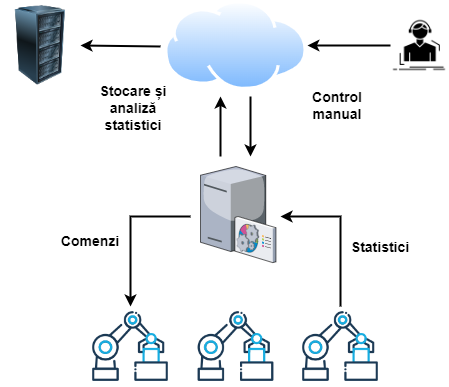
\includegraphics[width=0.9\textwidth]{images/exemplu_retea_iot_Cap3.drawio.png}
        \label{fig:exemplu_iiot}
    \end{minipage}\hfill
    \begin{minipage}{0.45\textwidth}
        \caption{Arhitectura \textit{3-layer} \\ (ilustrație adaptată după figura 1 din articolul \citetitle{Yousuf2015})}
        \centering
        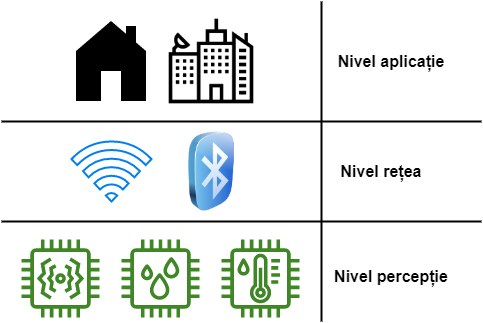
\includegraphics[width=0.9\textwidth]{images/3_layer.drawio.png}
        \label{fig:arch_3layer}
    \end{minipage}
\end{figure}

În continuare, ne vom concentra atenția asupra a trei modele arhitecturale populare în \acrshort{iot}, care oferă o abstractizare suficient de robustă pentru cazurile prezentate mai sus. Vor urma, astfel, în ordinea complexității, arhitectura \textit{3-layer}, \textit{5-layer} și \acrlong{soa}.

\subsection*{\textit{3-layer}}

\citet{MiaoWu2010} spune că în ciuda lipsei unei definiții unificate pentru \acrshort{iot}, arhitectura \textit{3-layer} este larg acceptată și cunoscută. Acest fapt este bine fundamentat, deoarece găsim referințe ale acestui model arhitectural în multiple publicații la care ne vom referi în paragrafele următoare. Mai jos sunt enumerate nivelurile componente ale acestei arhitecturi, iar în figura \ref{fig:arch_3layer} regăsim și o reprezentare grafică.

\begin{enumerate}
    \item Nivelul de percepție (\textit{perception layer})
    \item Nivelul rețelei (\textit{network layer})
    \item Nivelul aplicației (\textit{application layer})
\end{enumerate}

Nivelul de percepție conține senzori, cititoare de \acrshort{rfid} sau coduri de bare, sisteme \acrfull{gps} sau camere de filmat. Acesta facilitează colectarea de date despre mediul înconjurător al sistemului \acrshort{iot}. Identificăm cu ușurință acest nivel în exemplul nostru anterior, senzorii termici sau de mișcare, cât și dispozitivele de măsurat consumul de energie sau apă fac parte din acesta. Acest nivel poate fi considerat a fi colecția de \textit{things} din \acrshort{iot}.

La nivelul rețelei, întâlnim infrastructura care pune la dispoziție comunicarea dintre \textit{things}. Această infrastructură este formată din routere, \textit{switch}-uri, centre de procesare și management, etc. De exemplu, într-o locuință inteligentă rețeaua \textit{wireless} și centrul de control fac parte din nivelul de rețea.

Procesarea datelor și executarea fluxurilor specifice se petrece la nivelul aplicației. Acest nivel reprezintă totalitatea componentelor software și hardware, care facilitează serviciile dorite de utilizator. De exemplu, software-ul de automatizare, prezent pe centrul de comandă dintr-o locuință inteligentă, face parte din acest nivel.

\citet{Lin2017} constată că, deși această arhitectură este fundamentală și simplă, funcționalitățile și operațiunile desfășurate de sistem la nivelul rețelei și aplicației sunt diverse și complexe. În opinia autorilor, este nevoie de dezvoltarea unui nivel de serviciu (en. \textit{service layer}) care să medieze interacțiunea dintre rețea și aplicație. Acest nivel adițional ar facilita o mai mare flexibilitate sistemului.

\subsection*{\textit{5-layer}}

Arhitectura \textit{3-layer} nu conține metode de management suficient de bune și nu ia în considerare nevoia de a modela domeniile de \textit{business} în perspectiva lui \citet{MiaoWu2010}. Pentru a combate aceste dificultăți, autorii propun o arhitectura cu cinci nivele, după cum urmează:

\begin{enumerate}
    \item Nivelul de percepție (\textit{perception layer});
    \item Nivelul de transport (\textit{transport layer});
    \item Nivelul de procesare (\textit{processing layer});
    \item Nivelul aplicației (\textit{application layer});
    \item Nivelul \textit{business} (\textit{business layer}).
\end{enumerate}

Primele două nivele corespund cu cele din arhitectura \textit{3-layer}, îndeplinind aceleași funcții. În continuare, nivelul de procesare preia o parte din atribuțiile nivelului aplicației din arhitectura anterioară. Din acest nivel, fac parte bazele de date, \textit{cloud}-ul și toate celelalte aparaturi de procesare de date pentru a facilita utilizarea acestora la nivelul aplicației. În viziunea autorilor, această separare dintre procesare și utilizare în scopuri aplicate este necesară pentru flexibilitatea și scalabilitatea \acrshort{iot}.

În final, avem de a face cu nivelul de \textit{business}, care ar trebui să reprezinte un nivel de management peste nivelul aplicației, fiind preocupat de modelul de \textit{business} și dezvoltarea pe termen lung. Din păcate, autorii nu pun la dispoziție o descriere detaliată, aplicarea acestui tip de arhitectură rămânând la latitudinea dezvoltatorului. O imagine mai clară asupra nivelului de \textit{business} ne-o oferă \citet{Khan2012}, specificând că acesta conține modelele de \textit{business}, grafice și organigrame bazate pe datele obținute din nivelul de aplicație. Scopul acestui nivel este să producă strategii și decizii de \textit{business}, deci este un nivel de interacțiune între om și mașină.

\subsection*{\textit{Service Oriented Architecture}}

O arhitectură orientată pe servicii, în orginal \acrfull{soa}, propune împărțirea componentelor și funcționalităților unui sistem în unități mici și independente, numite servicii. Această arhitectură nu impune un număr fix de nivele, însă trebuie să existe cel puțin un nivel care facilitează două activități fundamentale: descoperirea serviciilor (\textit{service discovery}) și invocarea acestora (\textit{service calling}). 

\citet{Khodadadi2016} susțin că acest tip de arhitectură asigură interoperabilitatea dispozitivelor eterogene, această proprietate fiind esențială pentru sistemele \acrshort{iot}. De asemenea, oferă și un exemplu de \acrshort{soa}, adăugând un nivel de servicii în clasica arhitectură \textit{3-layer}. Funcționarea independentă a serviciilor asigură că sistemul va continua să funcționeze în general corect, chiar dacă un număr mic de servicii a încetat să funcționeze. Acest aspect este foarte important pentru fiabilitatea sistemelor. Același tip de arhitectură este descris și de \citet{Lin2017} într-un meta-studiu.

O altă perspectivă asupra unui posibil tip de \acrshort{soa} vine din partea lui \citet{LuTan2010}, care propun o arhitectură \textit{5-layer} modificată. Pe lângă nivelul rețelei, aceștia introduc un nivel de coordonare al serviciilor, care are rolul de a unifica comunicarea, asigurând interoperabilitatea. Din păcate, nu sunt oferite detalii suplimentare despre implementarea acestui tip de arhitectură.

\section{Protocoale de comunicație}

În discuția anterioară despre arhitectura sistemelor \acrshort{iot} am observat că un rol important este jucat de mecanismele de comunicare. Aceste sisteme sunt nevoite să coordoneze un număr mare de dispozitive și să transmită cantități enorme de date într-un mod fiabil, rapid și rezilient. De aceea sunt utilizate o gamă largă de protocoale de comunicație, fiecare cu avantajele și dezavantajele sale, în încercarea de a depăși provocările impuse de natura distribuită și eterogenă a sistemelor. În rândurile următoare, vor fi analizate o serie de protocoale utilizate în mod uzual. Vom trata protocoalele în ordine crescătoare, conform situării lor în modelul \acrshort{osi}. O ilustrație a acestui model se găsește în anexa \ref{apx:ilustratii}, figura \ref{fig:osi_model}.

Deoarece majoritatea comunicațiilor se desfășoară în mod \textit{wireless}, un protocol foarte popular pentru nivelul fizic și \textit{data link} este \textit{IEEE 802.15.4}. Așa cum ne spun \citet{Lin2017}, \textit{IEEE 802.15.4} este un protocol pentru comunicații cu consum scăzut de energie și rată mică de transfer. Datorită versatilității lui, acest protocol reprezintă baza pentru alte protocoale de nivel mai înalt precum \textit{ZigBee}, \textit{6LoWPAN} sau \textit{WirelessHART}, despre care vom vorbi în rândurile următoare.

Construit peste \textit{IEEE 802.15.4}, \textit{6LoWPAN} acoperă și nivelul de rețea \acrshort{osi}, folosind adresare \textit{IPv6}, astfel poate să ofere suport pentru rețele cu cost și consum de energie scăzute pentru un număr foarte mare de dispozitive \acrshort{iot}.

\textit{ZigBee} acoperă aproape toate nivelurile \acrshort{osi}, și anume: nivelul fizic, nivelul \textit{data link}, nivelul de rețea, de transport și cel al aplicației. Un avantaj foarte important al acestui protocol este posibilitatea de a crea topologii de rețea variate. Fiecare dispozitiv (nod) al rețelei poate juca rol de coordonator, router sau aplicație. Coordonatorul este punctul central al rețelei și atribuie rolurile router, acestea fiind responsabile pentru transmiterea pachetelor spre dispozitivele potrivite. Câteva exemple de topologii \textit{ZigBee} se pot observa în anexa \ref{apx:ilustratii}, figura \ref{fig:zigbee_networks}. O alternativă a acestui protocol este \textit{Z-Wave}, un protocol mult mai simplu, destinat rețelelor de mici dimensiuni (de până la 232 de noduri), oferind caracteristici similare în privința consumului de energie și ratelor de transfer de date.

Autointitulat protocolul principal pentru \acrshort{iot}, \acrfull{mqtt} este un protocol situat la nivelurile de sesiune și aplicație al \acrshort{osi}, destinat transmiterii de mesaje folosind modelul \textit{producător-consumator} (en. \textit{publisher-subscriber}). Acesta oferă reliziență și scalabilitate, fiind în același timp un protocol ”ușor” din punct de vedere al resurselor computaționale necesare. De asemenea, este potrivit pentru sistemele de tip \acrshort{eda}, categorie în care sistemele \acrshort{iot} se încadrează, după cum am discutat în capitolul al doilea. O alternativă pentru acest protocol este \acrfull{amqp}, însă acesta este mult mai complex și consumă, în general, mai multe resurse computaționale.

Probabil cel mai comun și cunoscut protocol de comunicație folosit în internet este \acrfull{http}. Acesta este utilizat și în cadrul sistemelor \acrshort{iot}, însă din cauza complexității acestuia și a faptului că este mult prea detaliat în specificarea cererilor, acesta nu este alegerea cea mai populară. În schimb, protocolul \acrfull{coap} este o versiune simplificată și optimizată pentru \acrshort{iot} a protocolului \acrshort{http}.

\section{Caracteristicile dispozitivelor hardware}

Am menționat anterior că spre deosebire de alte subdomenii ale tehnologiei informației, în \acrshort{iot}, software-ul este în strânsă legătură cu hardware-ul, uneori fiind inseparabile, deoarece nu există abstractizări hardware comune, utilizate de mai mulți producători. Vom menționa pe scurt care sunt principalele caracteristici ale dispozitivelor pe care le întâlnim în sistemele din piață:

\begin{itemize}
    \item \textbf{putere computațională mică} - senzorii, dispozitivele de control etc. au, în general, resurse computaționale foarte reduse, adică procesoare cu frecvențe de ordinul megahertzilor și memorii de ordinul \textit{kilobytes}-ilor;
    \item \textbf{lipsa capabilităților avansate de securitate} - facilități standard pe arhitecturi de procesoare pentru computere de uz personal, precum memoria neexecutabilă, unitatea de management a memoriei, etc., sunt inexistente pe foarte multe dispozitive \acrshort{iot};
    \item \textbf{lipsa de transparență} - codul sursă al programelor care rulează pe aceste dispozitive nu este disponibil, iar în multe cazuri, nu pot fi extrase programele în format binar (\textit{firmware}-ul nu este disponibil pentru public).
\end{itemize}

\section{Model teoretic}

În încercarea de a crea un cadru obiectiv pentru analiza sistemelor \acrshort{iot} din punct de vedere al proprietăților și potențialelor defecte din acestea, vom introduce câteva noțiuni teoretice pentru descrierea acestor sisteme. În secțiunea anterioară, am discutat despre comunicarea fizică a dispozitivelor, diferitele topologii pe care le-am putea întâlni și protocoalele utilizate. Vom extinde discuția spre fluxurile logice prezente în aceste rețele, deoarece, deși topologiile de tip stea sunt des întâlnite, nodul central servește ca un intermediar pentru fluxuri logice între un număr mare de dispozitive, acestea neputând fi reduse la o interacțiune nod central - dispozitiv.

Vom folosi ca fundație specificația propusă de \citet{Paduraru2021}, deoarece propune o descriere formală a rețelelor IoT, folosind teoria grafurilor pentru a ușura automatizarea proceselor de testare, fără a fi nevoie să se specifice detalii tehnice, precum protocoalele sau software-ul utilizat. Autorii propun să vizualizăm o aplicație IoT ca o serie de perechi \textit{input}-\textit{output}, care pot fi descrise de un graf orientat $G = (V, E)$ în modul următor:

\begin{enumerate}
    \item orice vârf $v \in V$ reprezintă un dispozitiv fizic, pe care se execută unul sau mai multe procese software;
    \item o muchie orientată $e \in E$ de la un vârf $v_1$ la un vârf $v_2$ descrie un flux de date de la \textit{output}-ul lui $v_1$ spre \textit{input-ul} lui $v_2$;
    \item orice vârf $v \in V$ este consumatorul datelor pentru un set de producători: 
        \begin{gather*}
            V_{in}(v) = \Big{\{} v_{in} \; \Big{|} \; \exists v \in V \land (v_{in}, v) \in E \Big{\}}
        \end{gather*}
    \item orice vârf $v \in V$ este producător pentru un set de consumatori:
        \begin{gather*}
            V_{out}(v) = \Big{\{} v_{out} \; \Big{|} \; \exists v \in V \land (v, v_{out}) \in E \Big{\}}
        \end{gather*}
    \item orice vârf $v \in V$ este caracterizat de un \textit{buffer} de \textit{input} și unul de \textit{output}, aceștia fiind descriși de relația între producător și consumator, astfel încât: 
        \begin{gather*}
            \mathrm{Buffer}_{in}(v) = \bigcup_{v_{in} \in V_{in}(v)} \mathrm{Buffer}_{out}(v_{in}) \\
            \mathrm{Buffer}_{out}(v) = \bigcup_{v_{out} \in V_{out}(v)} \mathrm{Buffer}_{in}(v_{out})
        \end{gather*}
    \item graful $G$ este dinamic, vârfuri și muchii putând fi adăugate sau eliminate în timpul funcționării rețelei.
\end{enumerate}

Un aspect important, discutat de autori, este că muchiile rețelei trebuie privite dintr-o perspectivă probabilistă, anume ele pot lipsi în timpul funcționării sistemului. De exemplu, un senzor ar putea fi deconectat, fără energie sau să comunice date la intervale foarte lungi de timp. O viziune mai clară asupra acestui aspect o putem avea privind figura \ref{fig:river_network}. În această figură, fluxurile de date ”curg” de la senzori spre nodurile de \textit{output} prin intermediul punctului central, \textit{hub}-ul rețelei. Observăm că unele muchii sau vârfuri din graf sunt obligatorii pentru funcționarea sistemului, eliminarea lor făcând imposibilă o execuție coerentă. Acest set de vârfuri și muchii obligatorii sunt notate $V_r$ și $E_r$ și determină graful funcțional minimal $G_r$. (ie. \textit{r} $\rightarrow$ \textit{required})

Dacă considerăm orice graf $G \in G_{total}$ o stare posibilă a rețelei (ie. $G$ conține toate muchiile și vârfurile obligatorii), observăm că avem de a face cu un automat finit. Putem descrie stările acestui automat, considerând $S = \Big{\{} G  \; \Big{|} \; G \in G_{total} \land G_{r} \subseteq G \Big{\}}$ și operațiile posibile de modificare ale grafului cărora le vom asocia următorul alfabet:
\begin{gather*}
    E^\oplus_e \coloneqq \text{adăugarea muchiei } e \;\;\;\; E^\ominus_e \coloneqq \text{ștergerea muchiei } e \\
    V^\oplus_v \coloneqq \text{adăugarea vârfului } v \;\;\;\; V^\ominus_v \coloneqq \text{ștergerea vârfului } v \\
    \\
    \Sigma = \Big{\{} E^\oplus_e \; \Big{|} \; e \in E_{total} \Big{\}} \bigcup
    \Big{\{} E^\ominus_e \; \Big{|} \; e \in E_{total}  \Big{\}} \bigcup \\
    \bigcup \Big{\{} V^\oplus_v \; \Big{|} \; v \in V_{total} \Big{\}} \bigcup
    \Big{\{} V^\ominus_v \; \Big{|} \; v \in V_{total} \Big{\}}
\end{gather*}

Folosind alfabetul definit mai sus, avem următoarea funcție de tranziție:

\begin{gather*}
    \delta(G = (V, E), E^\oplus_e) = G' = (V, E \cup \{e\}) \;\;\;\; \delta(G = (V, E), E^\ominus_e) = G' = (V, E \backslash \{e\}) \\
    \delta(G = (V, E), V^\oplus_v) = G' = (V \cup \{v\}, E) \;\;\;\; \delta(G = (V, E), V^\ominus_v) = G' = (V \backslash \{v\}, E)
\end{gather*}

Observăm că numărul de stări posibile ale acestui automat crește exponențial, mai exact proporțional cu numărul de submulțimi de vârfuri și muchii valide (totuși, număr mai mic decât $2^{|V| + |E|}$, deoarece nu toate combinațiile de vârfuri și muchii sunt valide).

\begin{figure}[h]
    \centering
    \caption{\centering Ilustrarea grafului orientat asociat unei rețele IoT, unde toate $S_i$ sunt senzori (\textit{input}), toate $F_i$ sunt noduri de ”filtrare”, $P_i$ sunt noduri de procesare, iar $O_i$ noduri de ieșire (\textit{output}). În centrul rețelei se află nodul central, denumit și \textit{hub}. Vârfurile și muchiile punctate reprezintă părți ale rețelei care pot lipsi. \newline (Ilustrație preluată din articolul \citetitle{Paduraru2021} al lui \citet{Paduraru2021})}
    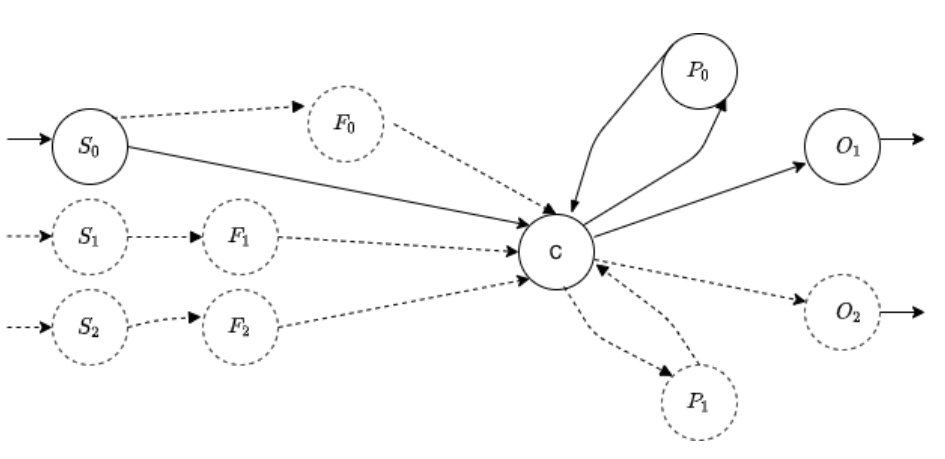
\includegraphics[width=0.9\textwidth]{images/river_topologie.png}
    \label{fig:river_network}
\end{figure}

O descriere mult mai precisă a sistemului ar putea fi reprezentată de utilizarea lanțurilor Markov, deoarece muchiile opționale au probabilități asociate, însă această abordare depășește scopul lucrării de față.

Descrierea propusă de \citet{Paduraru2021} se concentrează pe fluxurile fizice de date dintre dispozitive, însă un aspect important al acestor tipuri de sisteme este reprezentat de fluxurile logice de date, așa cum am văzut în discuția anterioară despre arhitecturi și protocoale, datele colectate de un senzor sau generate de un utilizator pot influența multiple părți ale sistemului, de la simplii actuatori până la sisteme complexe de analiză și decizie.

Într-o manieră similară celei de mai sus, putem descrie graful de fluxuri logice $G_L$ care conține aceleași vârfuri, însă nu și aceleași muchii. Deoarece abordarea este foarte similară, nu vom repeta notațiile propuse mai sus, dar vom analiza un scurt exemplu ilustrativ. Să presupunem că în figura \ref{fig:river_network} există o dependență logică între vârfurile $S_2$, $P_1$ și $O_2$. Atunci, în graful $G$ vor fi prezente muchiile: $S_2 F_2$, $F_2 C$, $C P_1$, $P_1 C$ și $C O_2$, deoarece datele nu pot urma alt drum fizic fără intermediarii $F_2$ și $C$. Pe de altă parte, în graful $G_L$ vor apărea doar muchiile determinate de drumul $S_2 P_1 O_2$, deoarece doar acestea iau parte la procesarea logică a fluxului de date.

Concluzionăm că am atins primul obiectiv al lucrării, anume stabilirea unui cadru tehnologic, dar și teoretic pentru sistemele \acrshort{iot}. Vom continua în capitolul următor cu descrierea modului în care am construit o suită de aplicații \acrshort{iot}, care să ilustreze cât mai bine caracteristicile tratate. Această suită va fi utilizată în finalul lucrării pentru evaluarea câtorva tehnici de testare.